\documentclass[doc, onecolumn, 12pt]{apa6}
\title{Deep Reinforcement Learning: Application of Deep Q-Networks and Deterministic Deep Policy Gradient to the Bipedal Walker Problem}
\usepackage{amsfonts}
\usepackage{amsmath}
\usepackage{setspace}
\usepackage{paralist}
\usepackage{hyperref}
\usepackage{amsfonts}
\usepackage{graphicx}
\usepackage[inline]{enumitem}
\usepackage[section]{placeins}
\usepackage{float}
\usepackage{grffile}
\usepackage{algorithm}
\usepackage{algpseudocode}
\restylefloat{table}
\usepackage[natbibapa]{apacite} 
\usepackage{graphicx}
\shorttitle{MSDS696: Practicum 2}
\affiliation{Regis University}
\author{Thomas Tarler\\ ttarler@gmail.com \\ (720) 496-9222}
\date{May  3rd 2020}
\begin{document}

\maketitle

\begin{abstract}


Reinforcement Learning is a type of machine learning which focuses on training an arbitrary agent to complete a complex task, such a a robot picking up a box. Deep reinforcement learning applies neural networks and deep learning to the reinforcement learning process. In this practicum, the author attempts to complete the Bipedal-Walker tasks using two algorithms: Deep-Q-Networks and Deep Deterministic Policy Gradients. The paper is practically split into two portions: 1) Theory and 2) Application. In Theory, we examine the mathematics behind Q-Learning and Reinforcement Learning, before diving into the specific mathematics of the algorithms we are employing. We then use a deep-learning cluster to train several agents to explore the behavior and performance of these models in practice. 

Due to the complexity of the models, the author's agents were never able to successfully complete a run. This may be to be expected as some of the algorithms are using up to four different neural networks. However we do yield interesting diagnostics data that is utilized to determine which model may be more successful in the long run. We finalize this paper with a simple explanation of potential business applications. 


\end{abstract}
\newpage
\tableofcontents
\newpage
\listoffigures
\newpage

Currently, many applications of data science rely on supervised and unsupervised learning models. These are tasks associated with labeling or predicting a value for a data set or attempting to ascertain an underlying structure to the data. The difficulty with models such as these is applying the results. For example, a model might suggest that a transaction has an 82\% probability of being fraudulent but it is up to the bank to decide what to do with that information. Reinforcement learning, on the other hand, focuses explicitly on actions or policies that an agent or actor can undertake in order to maximize some underlying profit function with respect to the environment. Mathematically, we describe this as \[ \mathcal{G} = \lbrace S_{i}, A_{i}, \Pi(S,A) \mapsto \mathbb{R} \rbrace\] where $\mathcal{G}$ is the game, $S_{i}$ is the state of agents and the environment, $A_{i}$ is the action set of the agent, and $\Pi$ is the profit function. The goal of reinforcement learning is to develop a set of rules, policies, or action-decisions that maximize the profit for a given agent. When principles of deep learning (i.e. neural networks) are applied to this framework, we refer to it as deep reinforcement learning. 

The author intends to use existing reinforcement learning frameworks and explore optimizing them against a game. The primary intention of this project is to compare the efficacy of deep reinforcement learning compared to techniques that do not utilize reinforcement learning. The intention is to explore and understand when deep-learning is more applicable to the problem, which has a faster training time, which performs better after a set number of training cycles, and other evaluation items. 

For this project, we will solve the OpenAI Bipedal Walker environment. This is a simulated physics environment where the goal is for the robot (the eponymous bipedal walker) to walk to the end of the environment. The game is initiated with no existing strategy or policy for the walker to complete the game, and it is deep reinforcement learning that yields the ability to complete the course. We chose this environment due to its intrinsic complexity and ability to compare multiple approaches. First, we will then examine the mathematics of Deep Reinforcement learning, with an overview of Augmented Random Search, Deep Q-Networks and Deterministic Deep Policy gradient. Finally we will demonstrates completed successful runs using various different models. We will then offer a detailed explanation of the Bipedal Walker game and associated components. We will conclude this project with a quick overview of our training results. 

Due to the complex computational needs of this exercise, all major iterations have been completed on the Regis University Deep Computing cluster, which does not support the .ipynb format. Wherever possible we will include the scripts that we ran at the end of this document or otherwise linked but will not display code and results.


\section{Theory}
As opposed to Supervised Learning and Unsupervised learning, reinforcement learning does not deal with the traditional mathematical constructs of a data set with either some label, value, or underlying structure associated with it. Nor do we evaluate models produced in the traditional manner; there is no binary classification or topological metric that we can use to satisfy business requirements. Rather, reinforcement learning is concerned with some task that an agent may or may not complete using one or more actions. The agent is graded using an award function, and is typically competing against other agents or the environment. As such the central mathematical construct for reinforcement learning is game theory. For this theory section of the paper, the author will walk through what is reinforcement learning and then give details around the various algorithms used to solve a reinforcement learning task. 
\subsection{Reinforcement Learning}
There are two entities involved within reinforcement learning: the agent or actor, and the environment The agent, $\mathcal{A}$ has a state and a set of actions associated with it. The is opposed to the environment which only has its state and future encoded states associated with it Beyond there agent and environment framework: there are four central components, the policy, the reward signal, the value function, and the model of the environment. It is important to step through all of these components mathematically before delving into the specific algorithms and problems we are trying to solve. 

Within each agent, we have an associated set of states, $s$ at each time step. That is, $S = \lbrace s_{1}, s_{2}, \ldots, s_{t-1}, s_{t} \rbrace$ represents all possible states associated with an agent. We have implicitly defined with time $t$ represents a set of steps, however states are not necessarily linear in time. A policy, $p$ then maps an action, $a_{i}$ and a state associated with an actor to a new state. That is, $p: s_{i} \times a_{i} \mapsto s_{j \neq i}$. The goal of reinforcement learning is to find the optimal policy, $p_{i}$ for a given actor and state. 


The reward signal is vital for determining how good a policy and/or state is. We define the reward signal, $r$ to be the function that takes an agents state and maps it to a number. That is, $r: A_{i} \times S(A_{i})_{t} \mapsto \mathbb{R}$ where $S(A_{i})_{t}$ signifies the state associated with a given actor at time $t$. 

The valuation function defines very specifically how a given reward is valued over time, or until the end of the game. This enables the agent to consider their total possible award for the rest of the game and ensures that long-term strategic thinking is employed. At its basic, we define it as $$V(A_{i}) = \sum_{t_{a}}^{t} R(A_{i}, S(A_{i})_{t} $$ but in practice often  includes a discount function to factor in present and future value. An agent will seek to maximize this value function for the remainder of the game. If the value function is relatively low, then agent may take a \emph{riskier} set of policies to maximize their success or failure. 

Finally, we need the environment or the model of an environment.  The environmental model represents the state of the environment for a given time $t$ and enables future planning for possible actions in an environment and enables an agent to calculate our their future earnings and actions given potential changes to the state of the environment. The environment can also encode the actions of other, either adversarial or cooperative agents in order to facilitate the actions of others upon an agent. This is where the OpenAI gym comes in handy, in that it simulates an arbitrary environment - in this case a two-dimensional physics world. 

\subsection{Deep Q-Networks}
Deep Q-Networks are a variation on Q-Learning and so we will explain Q-Learning first. Q-learning is explicitly \emph{model-free} meaning that no agent encodes a model of the environment they are working on, Instead each state is considered to be a step in a Markov Chain, so that the state can always be calculated using the last observation. Q-learning attempts to determine an optimal policy $Q$ for a given agent and action-state combination. Note that each action-state must be discrete and enumerated, meaning we can associated indices $i, j \in \mathbb{N}$ with every action state, and the size of Q-Learning is $i \cdot j$. We first need to define the valuation function as 
\begin{equation} 
\label{bellman}
Q^{\prime}(s_{t}, a_{t}) \leftarrow Q(s_{t}, a_{t}) + \alpha \cdot \left( r_{t} + \gamma \cdot \max_{\alpha} Q(s_{t+1}, a_{t}) - Q(s_{t}, a_{t}) \right)
\end{equation}  where $Q^{\prime}$ is the updated policy, $\gamma \in \mathbb{R} \cap [0,1]$ is the \emph{discount} rate (or how much the model discount future values to the prevent), $\alpha \in \mathbb{R} \cap [0,1]$ is the \emph{learning rate} (how much the model learns from past actions) and $r_{t}$ is the present reward at time $t$.  Necessarily, setting $\gamma$ low means the model does not discount future actions as much and disregards actions that may improve its current state for a longer-term reward. Conversely, setting $\gamma$ high means future actions are heavily discounted and the model becomes greedy. When we set $\alpha$ to a low value, the model with not learn as much from its future actions and will bias itself towards using past, successful actions. When $\alpha$ is high, the model will learn more. A final variable that is vital is $\epsilon \in \mathbb{R} \cap [0,1]$ or the experimentation rate. If $\epsilon$ is high, the model will chose to undertake a completely random action more frequently rather than some policy it has already learned to be successful. 

Equation \eqref{bellman} is the cost function traditionally used in both Q-Learning and Deep-Variants. It is known as the Bellman equation. 

Traditionally, Q-Networks have been trained using somewhat of a brute-force approach, where nearly every action and state combination. This means when states or actions gets very large, the efficacy of Q-Learning diminishes.  For the agent to be successful, every state must have been experienced and every possible sequence of actions must also have been undertaken. Deep Q-Networks relax this assumption by allowing very large action-state combination spaces, though they must be discrete in nature. That is, there are still a finite (but very large) number of action-state combinations. This means that the Q-Learner is replaced with a neural network of some sort, $Q: S \mapsto A$ which takes in the state of the environment and outputs a suitable action. Since neural networks can be used to approximate nearly an function $f$ this means that the action of training a neural network can approach a more efficient learner than the brute force approach. Other than using a neural network to determine the best policy, Deep Q-Networks are otherwise homeomorphic to traditional Q-Learning. 

\begin{algorithm}[H]
\caption{ DQN Algorithm \citep{DBLP:journals/corr/MnihKSGAWR13}}
\begin{algorithmic}[1]
\State Initialize Replay memory $\mathcal{D}$ to capacity $\mathcal{N}$
\State Initialize Action-Value function $Q$ with random weights 
\For {episode = 1,M} 
	\State Initialize Sequence $s_{i} = \lbrace x_{i} \rbrace$ and preprocessed sequence $\phi_{1} = \phi(s_{1})$
	\For {$t=1,T}$ 
		\State with probability $\epsilon$ select a random action $a_{t}$
		\State otherwise select $a_{t} = \max_{a} Q^{\star} (\phi(s_{t}), a; \theta)$
		\State Execute action $a_{t}$ and observe reward $r_{t}$ and image $x_{t+1}$
		\State Set $s_{t+1} = s_{t}, a_{t}, x_{t+1}$ and preprocess $\phi_{t+1}=\phi(s_{t+1})$
		\State Store transaction $(\phi_{t}, a_{t}, r_{t}, \phi_{t+1})$ in $\mathcal{D}$
		\State Sample random mini batch of transactions $(\phi_{j}, a_{j}, r_{j}, \phi_{j+1})$ from $\mathcal{D}$
		\State Set \[y_{i} = 
		\left\{\begin{array}{lr}
		
		 r_{j}  & \text{for terminal }  \phi_{J+1} \\
		r_{j} + \gamma  \max_{a ^{\prime}} Q^{\star} (\phi_{j+1}, a^{\prime}; \theta^{\prime})  &  \text{for non-terminal}  \phi_{J+1} 
		\end{array} \right\}
		\]
		\State Perform a gradient descent step on $(y_{j}-Q(\phi_{j},a_{j}; \theta))^{2}$
	\EndFor

\EndFor
\end{algorithmic}
\end{algorithm}
\FloatBarrier

There are two key distinctions between Q-Learning and a Deep-Q-Network: The experience replay buffer and the actor-network. The Experience replay buffer is necessary because sequential experiences tend to be correlated. That is $s_{t} ~ s_{t+1}$ and so on.  We want these experiences to be independently distributed so that the Actor-network may gain a better understanding of what causes each $s_{t}$. Therefore we randomly sample from the replay buffer $\mathcal{D}$ and use a preimage process to de-correlate of $\phi_{i} = \phi(s_{i})$. 

The actor-network is a typical neural network, what is critical is how we perform gradient descent in order to facilitate backward propagation. We then take equation \eqref{bellman} and define a loss function \begin{equation}
\label{loss-dqn}
L(\theta_{i}) = \mathbb{E}  \left[ (y_{i} -Q(s,a;\theta_{i}))^{2} \right]
\end{equation} 
where \begin{equation} \label{y-loss}
y_{i} = 
		\left\{\begin{array}{lr}
		 r_{j}  & \text{for terminal }  \phi_{J+1} \\
		r_{j} + \gamma  \max_{a ^{\prime}} Q^{\star} (\phi_{j+1}, a^{\prime}; \theta^{\prime})  &  \text{for non-terminal}  \phi_{J+1} 
		\end{array} \right\}
\end{equation}
We can then take the derivative of \eqref{y-loss} and yield \begin{equation}
\label{loss-actor}
\nabla_{\theta_{i}} = \mathbb{E} \left[R_{t+1} + \gamma \max_{a^{\prime}} Q(s_{t+1},a^{\prime})-Q(s,  a; \theta_{i}))\nabla_{\theta_{i}}Q(s,a; \theta_{i} \right] 
\end{equation}

\FloatBarrier
\subsection{Deep Deterministic Policy Networks}
The Deep Deterministic Policy Networks (DDPG) are a further refinement to Deep Q-Networks however they relax the assumption that states and actions must be discrete and instead account for \emph{continuous} states and actions. This means that while the input and output dimensions are still categories, the value encoded within them reverts from some boolean value (e.g. Is there an actor in space $(n,m)$) to continues (e.g. what is the probability that there is an actor in space $(n,m)$. 

\begin{algorithm}[H]
\caption{DDPG Algorithm \citep{DDPG}}
\begin{algorithmic}[1]
\State Randomly initialize critic network $Q(s, a \vert \theta^{Q})$ and actor $\mu(s \vert \theta^{\mu})$ with weights $\theta^{Q}$ and $\theta^{\mu}$
\State Initialize target network $Q^{\prime}$ and $\mu^{\prime}$ with weights $\theta^{Q^{\prime}} \leftarrow \theta^{Q}$, $\theta^{\mu^{\prime}} \leftarrow \theta^{\mu}$
\State Initialize replay buffer R
\For{episode = 1, M} 
	\State Initialize  a random process $\mathcal{N}$ for action exploration 
	\State Receive initial observation state $s_{1}$
	\For {t = 1, T}
		\State Select action $a_{t}= \mu(s_{t} \vert \theta^{\mu}) + \mathcal{N}_{1}$ according to the current policy and exploration noise
		\State Execute action $a_{t}$ and observe reward $t_{t}$ and observe new state $s_{t+1}$ 
		\State Sample a random mini batch of $N$ transitions $(s_{i}, a_{i}, r_{i}, s_{i+1})$ from $R$
		\State Set $y_{I} = r_{i} + \gamma Q^{\prime}(s_{i+1}, \mu^{\prime}(s_{i+1} \vert \theta^{\mu^{\prime}} ) \vert \theta^{Q^{\prime}})$
		\State Update critic by minimizing the loss $L= \frac{1}{n}\sigma_{i}(y_{i}-Q(s_{i},a_{i} \vert \theta^{Q}))^{2}$
		\State Update the actor policy using the sampled policy gradient: \[ \nabla_{\theta \mu} J \approx \frac{1}{N} \sum_{i} \nabla_{a} Q(s, a \vert \theta^{Q}) \vert_{s=s_{i}, a = \mu (s_{i})}  \nabla_{\theta\mu} \mu(s \vert \theta ^{\mu}) \vert s_{i} \]
		\State Update the target networks: 
			\[\theta^{Q^{\prime}} \leftarrow \gamma\theta^{Q} + (1- \gamma)\theta^{Q^{\prime}} \] 
			\[ 			\theta^{\mu^{\prime}} \leftarrow \gamma\theta^{\mu} + (1- \gamma)\theta^{\mu^{\prime}}  \]
	\EndFor
\EndFor
\end{algorithmic}
\end{algorithm}


A a very high level, the  DDPG take advantage of four different and diverse networks: \begin{enumerate}
\item $\theta^{Q}$  is the \emph{Actor-Critic} network, where an actor or agents actions are criticized by a critic for good output, similar to GAN
\item $\theta^{\mu}$ is the deterministic policy network, a neural network that determines best possible action given a time, and serves as long-term memory
\item $\theta^{Q^{\prime}}$ Target Q-Network, a Time-delayed version $\theta^{Q}$
\item $\theta^{\mu^{\prime}}$ Target-policy network, a time delayed version of the policy network
\end{enumerate} 

The actor-critic network is similar to a GAN architecture. Since there is no \emph{label} to be applied with this type of learning, the Critic network is meant to tell the actor how good their policy/action is prior to a reward function being calculated. There are four components to explore within this: Replay Buffer, Actor and Critic Updates, target network updates, and Exploration. 

The Replay Buffer is almost identical to the DQN network above, and we will not explore. Similar to above, there is a tuple of $(s_{i}, a_{i}, r_{i}, s_{i+1})$ that are randomly sampled to be used and create linearly independent states.

Similar to Deep Q-Networks, the Actor network (which focuses on policy) is updated using a discounted future-state value of rewards, though with target value (critic) and target policy networks. Equations \eqref{loss-actor} and \eqref{loss-dqn} cover these.  However the Critic Network is the first significant difference from DQN. The crittic network contains the policy function \begin{equation} \label{policy} 
J(\theta) = \mathbb{E}  \left[ Q(s,a) \vert_{s=s_{t}a=\mu(s_{t}} \right]
\end{equation} 

Since this is a well-defined function, all we have to do for the loss is to take the dertivate of the Policy function  \eqref{policy} with respect to the policy parameter. That is:  \begin{equation} \label{polderiv}  \nabla_{\theta \mu} J \approx \frac{1}{N} \sum_{i} \nabla_{a} Q(s, a \vert \theta^{Q}) \vert_{s=s_{i}, a = \mu (s_{i})}  \nabla_{\theta\mu} \mu(s \vert \theta ^{\mu}) \vert s_{i} \end{equation}

Target Network updates are then performed where we take a copy of $\theta^{Q}$ and $\theta^{\mu}$ and update them with a parameter $\tau$. This allows for a slower \emph{learning} of these networks that takes place on a greater scale than epochs and episodes. 

The final important aspect is exploration. In discrete reinforcement learning problems, we can chose a random action $a_{i}$ from the action space whenever $\epsilon_{i} < \epsilon$. This is important to learn new actions. However in a continuous action space, we instead want to inject random noise into an action. For example, moving a joint just slightly harder. DDPG networks use the \emph{Urnstein-Uhlenbeck Process} for the noise to ensure that it does not cancel an action. This process is \[ \mu ^{\prime}(s_{t}) = \mu( s_{t} \vert \theta^{\mu}_{t}) + \mathcal{N}\]



\newpage
\section{Bipedal Walker}
The Bipedal Walker is a continuous game made available by OpenAI. Like any game, there are two primary components, the environment and the agent, with the two coupled together in a profit or reward function. That is, an \textbf{agent} takes an action. This action has a tangible effect on the \textbf{environment} and the state of the agent. If the action results in a favorable movement in the environment, then the agent is given a positive award. 

We will first examine the agent, or the bipedal walker. The Bipedal Walker or $\mathbb{A}$ has two distinct attributes: the action space $\mathcal{A}$ and the observation space $\mathcal{O}$. In general, our neural network is a function, $D$ such that $D: \mathcal{O} \mapsto \mathcal{A}$.  

The observation space for the robot is rather large, that is $\vert \mathcal{O} \vert = 24$. That is, there are twenty-four different observations that the agent can make about itself (numbers 0-13) and about the environment using its Lidar (14-23).  

\begin{table}[H]
\begin{tabular}{|l|l|l|l|l|}
\hline
Num   & Observation                   & Min  & Max  & Mean \\ \hline
0     & hull\_angle                   & 0    & $2 \pi$ & 0.5  \\ \hline
1     & hull\_angularVelocity         & -$\infty$ & +$\infty$ & -    \\ \hline
2     & vel\_x                        & -1   & +1   & -    \\ \hline
3     & vel\_y                        & -1   & +1   & -    \\ \hline
4     & hip\_joint\_1\_angle          & -$\infty$& +$\infty$& -    \\ \hline
5     & hip\_joint\_1\_speed          & -$\infty$ & +$\infty$& -    \\ \hline
6     & knee\_joint\_1\_angle         & -$\infty$& +$\infty$& -    \\ \hline
7     & knee\_joint\_1\_speed         & -$\infty$& +$\infty$& -    \\ \hline
8     & leg\_1\_ground\_contact\_flag & 0    & 1    & -    \\ \hline
9     & hip\_joint\_2\_angle          & -$\infty$& +$\infty$& -    \\ \hline
10    & hip\_joint\_2\_speed          & -$\infty$& +$\infty$& -    \\ \hline
11    & knee\_joint\_2\_angle         & -$\infty$& +$\infty$& -    \\ \hline
12    & knee\_joint\_2\_speed         & -$\infty$& +$\infty$& -    \\ \hline
13    & leg\_2\_ground\_contact\_flag & 0    & 1    & -    \\ \hline
14-23 & 10 lidar readings             & -$\infty$& +$\infty$& - \\  \hline
\end{tabular}
\end{table}

In the Bipedal Walker, the size of the action space is A or $\vert \mathcal{A} \vert = 4$ with each action corresponding to some joint (two knees, two hips). For each $i \in \mathbb{Z} \cap 4$, there is a torque associated with it. Hence we have

\begin{table}[H]
\begin{tabular}{|l|l|l|l|}
\hline
Num & Name   & Min & Max \\ \hline
0   & Hip 1  & -1  & +1  \\ \hline
1   & Knee 1 & -1  & +1  \\ \hline
2   & Hip 2  & -1  & +1  \\ \hline
3   & Knee 2 & -1  & +1  \\ \hline
\end{tabular}
\end{table}

The goal of the bipedal walker is to train the robot to complete the course. The reward function $R(t)$ is defined as the following: 
\[ R(t) = \left \{\begin{array}{lr}
 300 & \text{Walker completes course} \\
 -100 & \text{Walker falls down} \\
 -x & \text{Seconds where torque is applie to the motor} 
\end{array}\right\}  \]

This creates an easy to see victory condition, that is when $R> 300$. The specific structure of the cost function is such that the best performing Robot walkers will not only complete the course in a minimum of time, but will also have the smallest amount of energy used for walking.
The starting position of the simulation is with the robot at the far left of the course with mostly straight legs. The failure condition is when the hull-contact sensor touches ground (the robot has fallen) or the stage has been complete.  Please reference figure \ref{biped}  on \pageref{biped} for a visual diagram of the environment. 

\begin{figure}[H]

\caption{Bipedal Walker Environment}
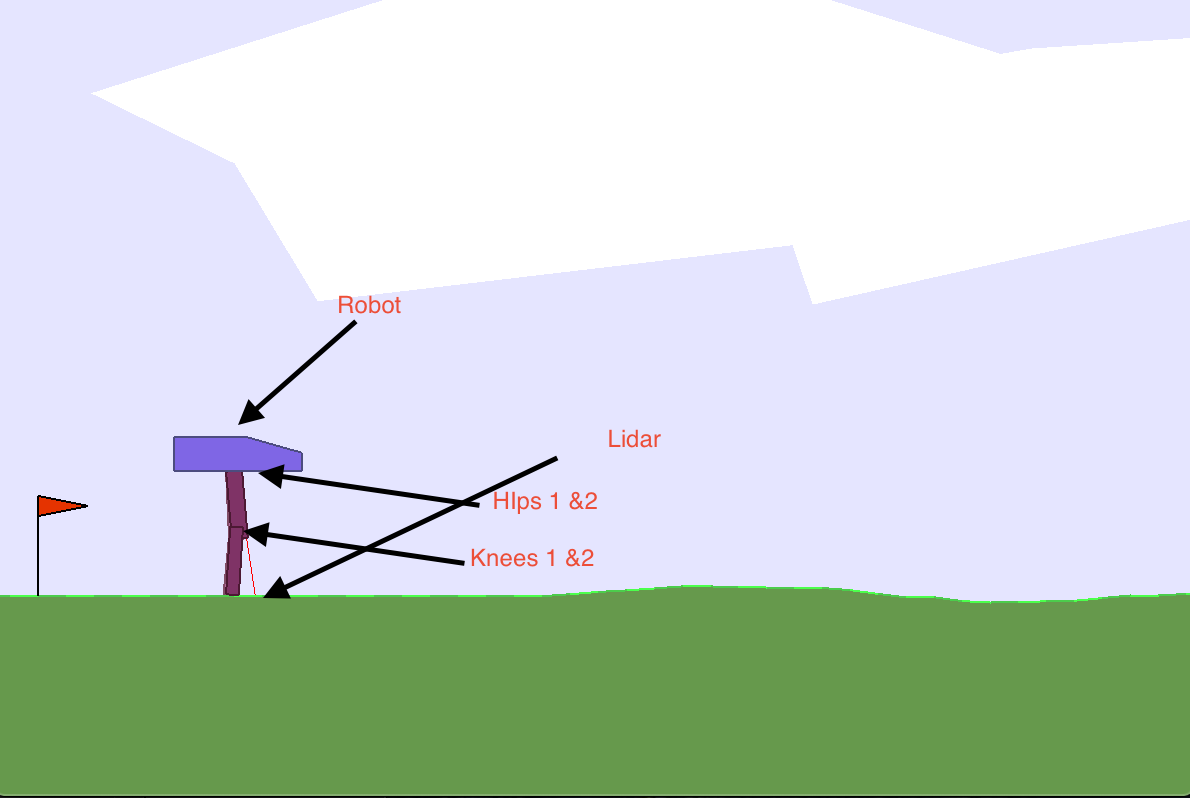
\includegraphics[width = \textwidth]{bipedal.png}
\label{biped}
\end{figure} 
\FloatBarrier
\clearpage
\section{Results}
\subsection{Methodology}
For both the DQN and the DDPG, training was done on a remote Regis cluster with three GPU's and job management. These clusters were built without a GUI interface. To begin with, results were run with the episodes and epochs setting set to 10000 each with model checkpoints as applicable.

Code was implemented from the [insert] repositories. Code was tweaked to run on the Regis University cluster, with parameters changed around environment rendering, save-states and V1 vs. V2 implementations. The neural networks were minority tweaked to get them operating and returning results. 

\subsection{DQN}
The following hyperparameters were used for DQN networks. \begin{itemize}
\item $\gamma = 0.98$
\item $\alpha_{agent} = 0.02$
\item $\epsilon_{\text{initial}} = 1.0$\footnote{$\epsilon$ varies throughout based on a decay rate of $0.995$} 
\end{itemize}

Additionally, we had a simple sequential model for the DQN, as shown in Figure \ref{DQN_Architecture} on page \pageref{DQN_Architecture}.

\begin{figure}

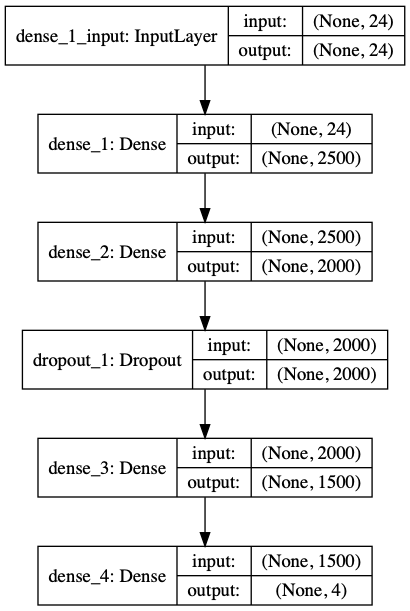
\includegraphics[width=\textwidth]{results/dqn/DQN_Model.png}
\caption{Neural Architecture of the DQN Model used for training}
\label{DQN_Architecture}
\end{figure}

\FloatBarrier
\subsubsection{1000 Episodes}
\begin{figure}[H]
\label{DQN_1000Ep_Error}
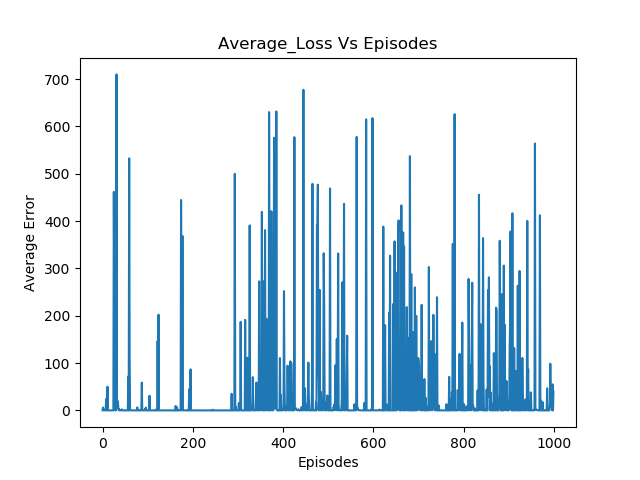
\includegraphics[width =\textwidth, height=0.4 \textheight]{results/dqn/1000_ep/Error.png}
\caption{Loss and Error when DQN is run for 1000 Episodes}
\end{figure}

\begin{figure}

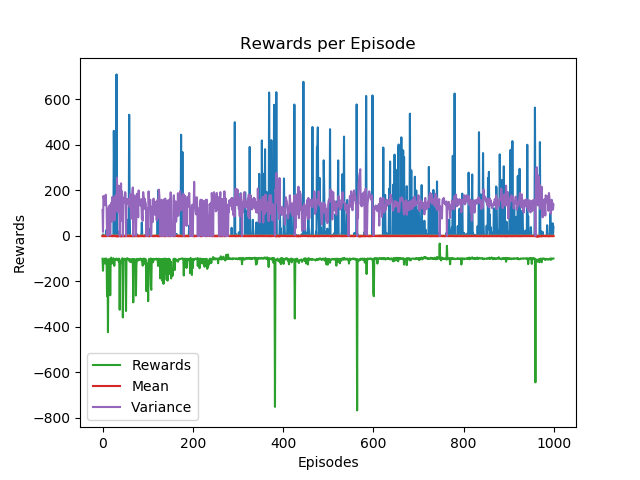
\includegraphics[width =\textwidth, height=0.4 \textheight]{results/dqn/1000_ep/Rewards.png}
\caption{Reward  when DQN is run for 1000 Episodes}
\label{DQN_1000Ep_Rewards}
\end{figure}

\begin{figure}

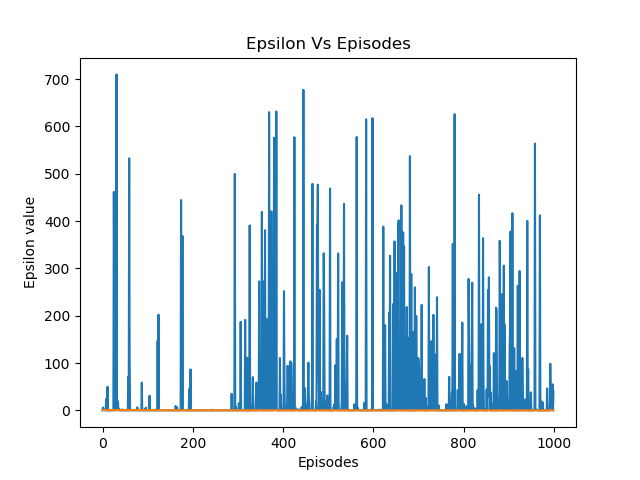
\includegraphics[width =\textwidth, height=0.4 \textheight]{results/dqn/1000_ep/Epsilon.png}
\caption{Epislon when DQN is run for 1000 Episodes}
\label{DQN_1000Ep_Epsilon}
\end{figure}

\FloatBarrier 
\subsubsection{5000 Episodes}
\begin{figure}
\label{DQN_5000Ep_Error}
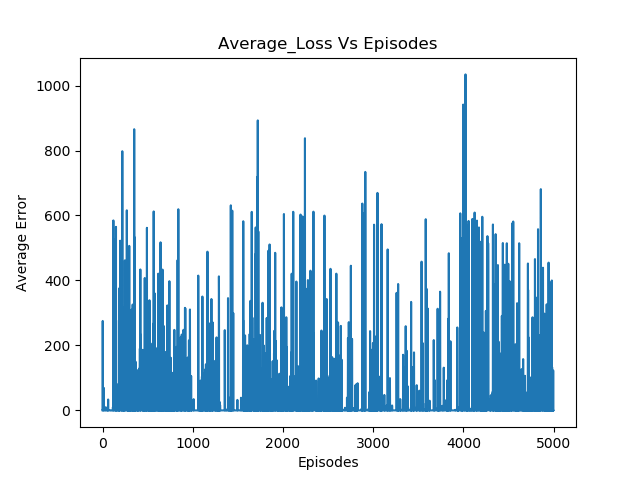
\includegraphics[width =\textwidth, height=0.4 \textheight]{results/dqn/5000_ep/Error.png}
\caption{Loss and Error when DQN is run for 5000 Episodes}
\end{figure}

\begin{figure}
\label{DQN_5000Ep_Rewards}
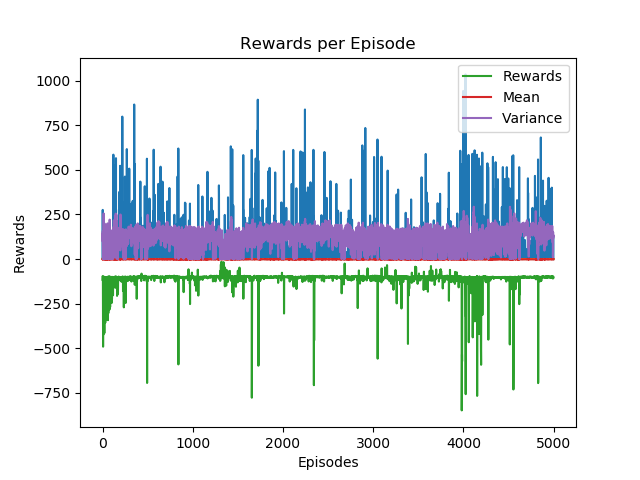
\includegraphics[width =\textwidth, height=0.4 \textheight]{results/dqn/5000_ep/Rewards.png}
\caption{Reward  when DQN is run for 5000 Episodes}
\end{figure}

\begin{figure}
\label{DQN_5000Ep_Epsilon}
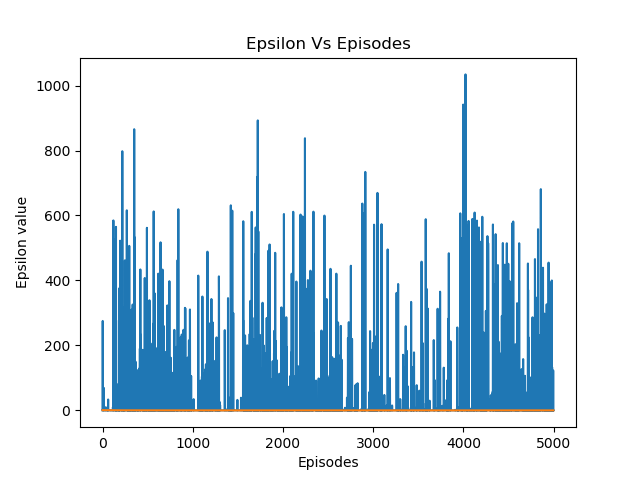
\includegraphics[width =\textwidth, height=0.4 \textheight]{results/dqn/5000_ep/Epsilon.png}
\caption{Epsilon when DQN is run for 5000 Episodes}
\end{figure}

\FloatBarrier 



\subsection{DDPG}

The following hyperparameters we used for the DDPG networks. \begin{itemize}
\item $\gamma = 0.85$
\item $\alpha_{agent} = 0.1$
\item $\alpha_{critic} = 0.02$
\item $\hat{\alpha} = 0.1$ 
\item $\tau = 0.01$
\item $\epsilon_{\text{initial}} = 1.0$\footnote{$\epsilon$ varies throughout, similar to DQN, and is governed by the Ornstein Uhlenbeck Process} 
\end{itemize}

The four networks used in the DDPG are listed below: 

\begin{figure}
\label{DDPG_ActorLocal}
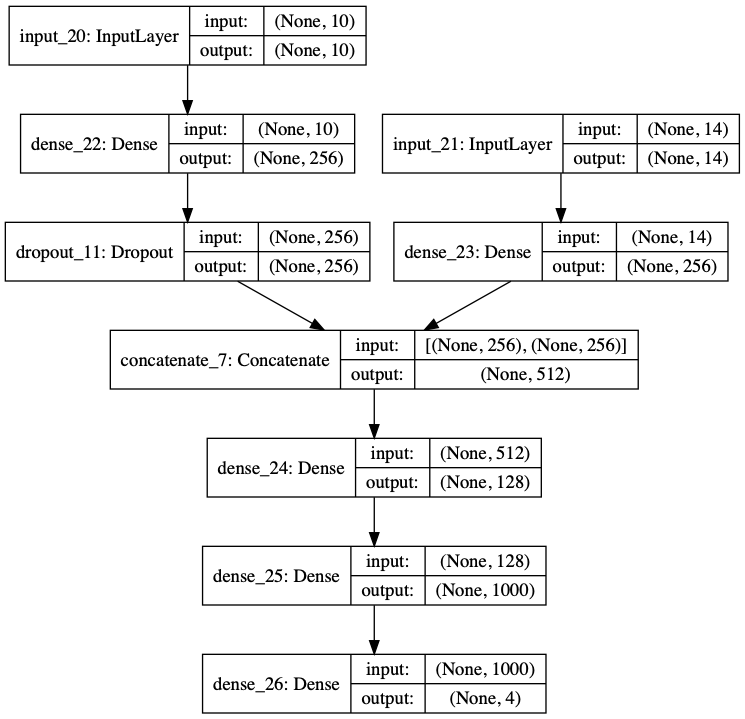
\includegraphics[width=\textwidth]{results/ddpg/DDPG_Actorlc.png}
\caption{DDPG Actor Local Network}
\end{figure}


\begin{figure}
\label{DDPG_ActorTarget}
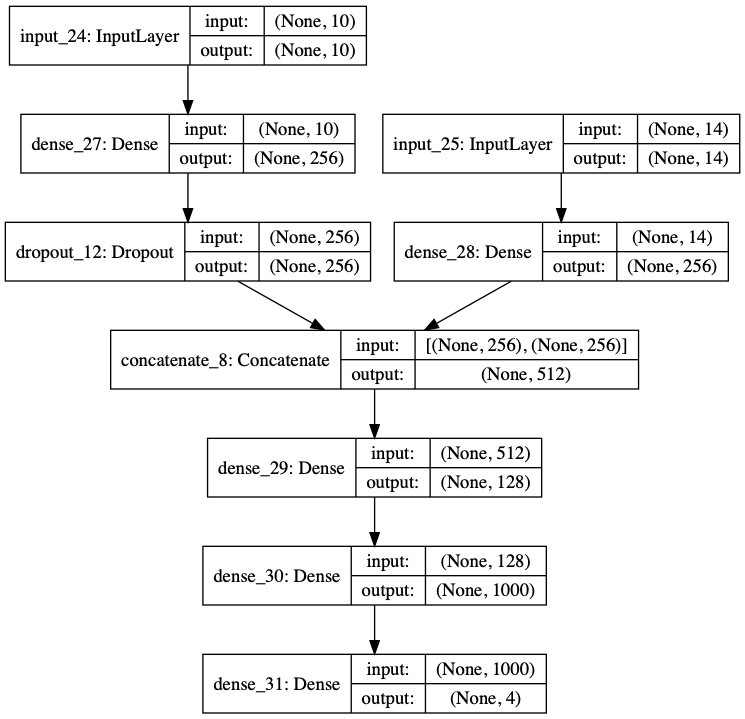
\includegraphics[width=\textwidth]{results/ddpg/DDPG_Actortg.png}
\caption{DDPG Actor Target Network}
\end{figure}

\begin{figure}
\label{DDPG_CriticLocal}
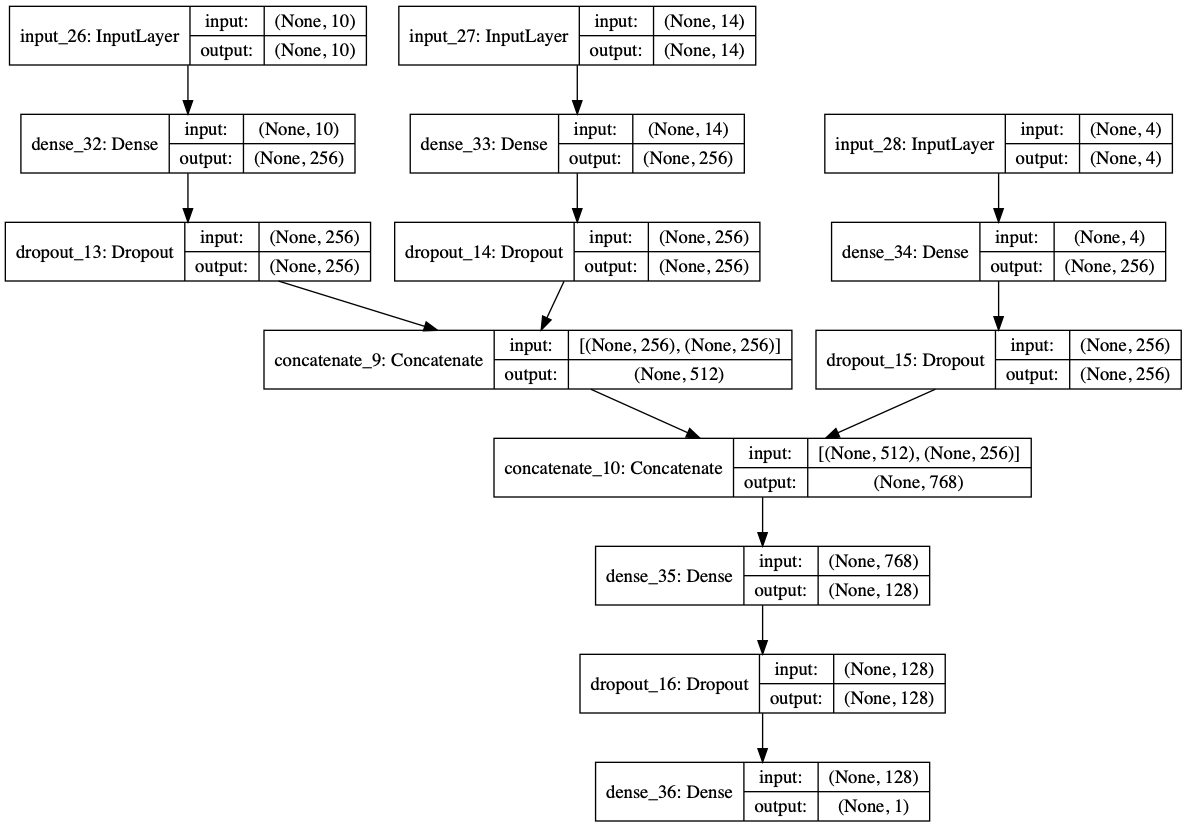
\includegraphics[width=\textwidth]{results/ddpg/DDPG_critictlc.png}
\caption{DDPG Critic Local Network}
\end{figure}

\begin{figure}
\label{DDPG_CriticTarget}
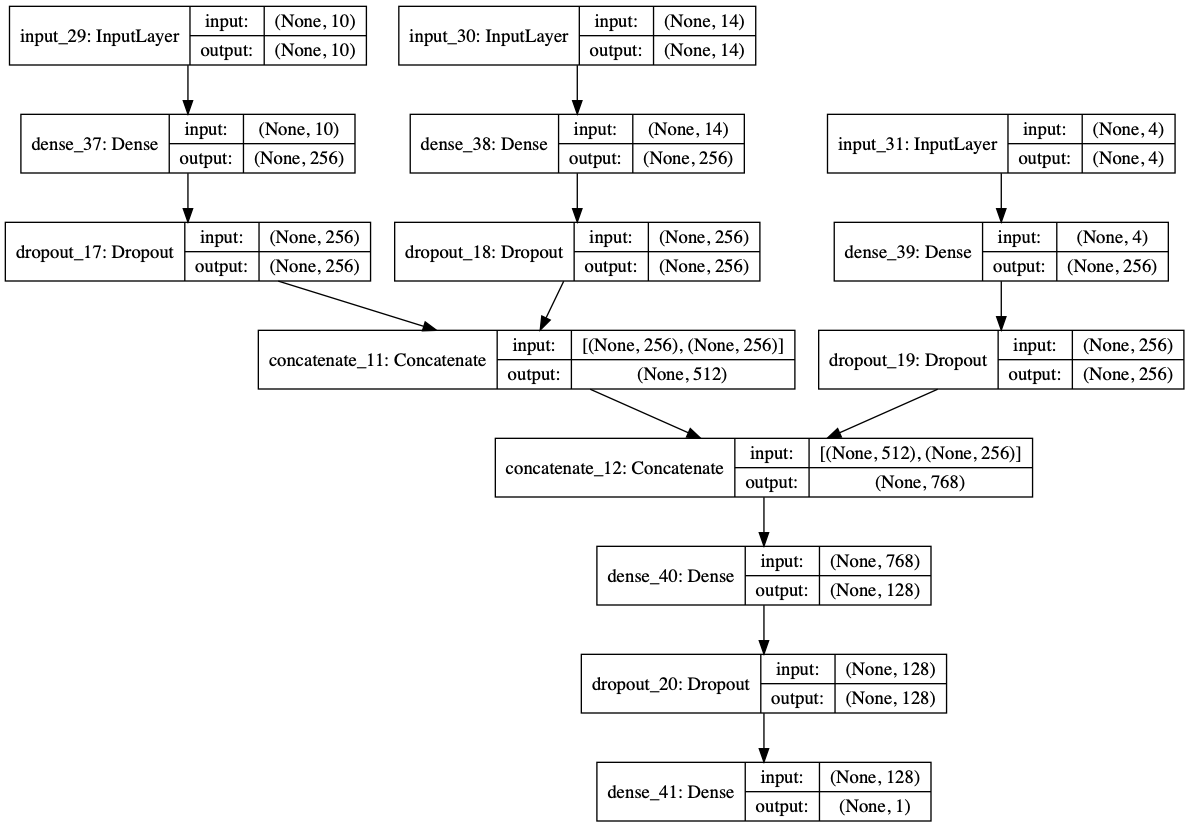
\includegraphics[width=\textwidth]{results/ddpg/DDPG_critictg.png}
\caption{DDPG Critic Target Network}
\end{figure}



\FloatBarrier
\subsubsection{1000 Episodes}

\begin{figure}
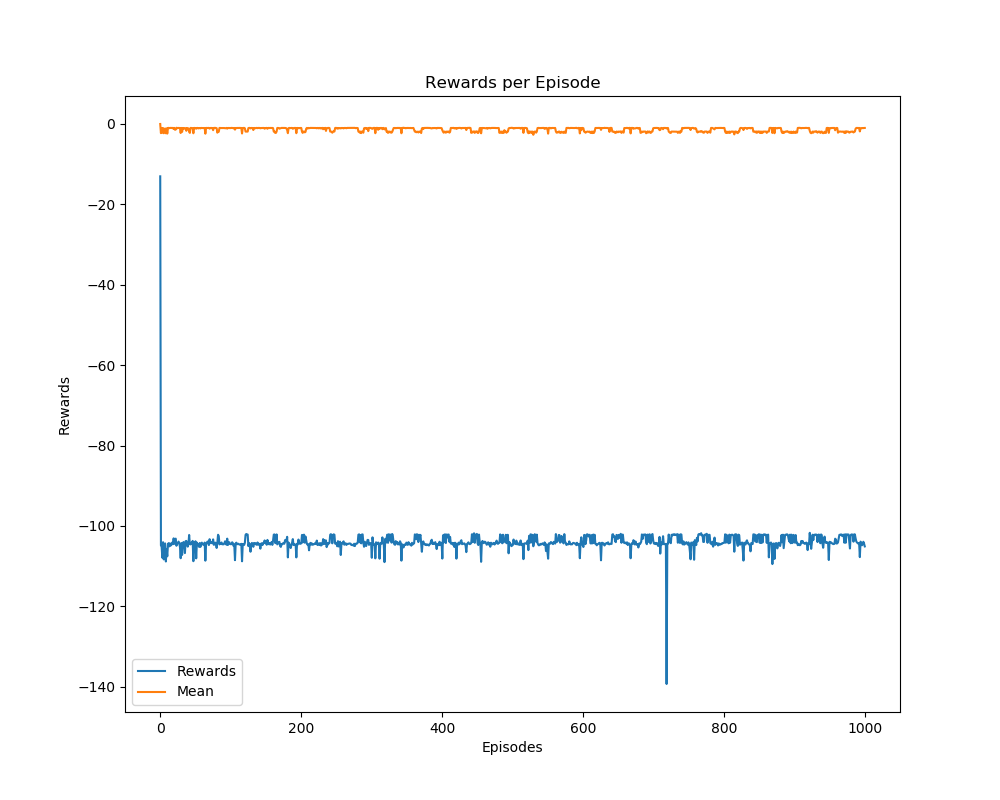
\includegraphics[width =\textwidth, height=0.4 \textheight]{results/ddpg/1000_ep/Rewards.png}
\caption{Reward when DDPG is run for 1000 Episodes}
\label{DDPG_1000Ep_Rewards}
\end{figure}

\begin{figure}

\includegraphics[width =\textwidth, height=0.4 \textheight]{results/ddpg/1000_ep/Epsilon.png}
\caption{Epislon when DDPG is run for 1000 Episodes}
\label{DDPG_1000Ep_Epsilon}
\end{figure}

\FloatBarrier 

\subsubsection{5000 Episodes}


\begin{figure}
\label{DDPG_5000Ep_Rewards}
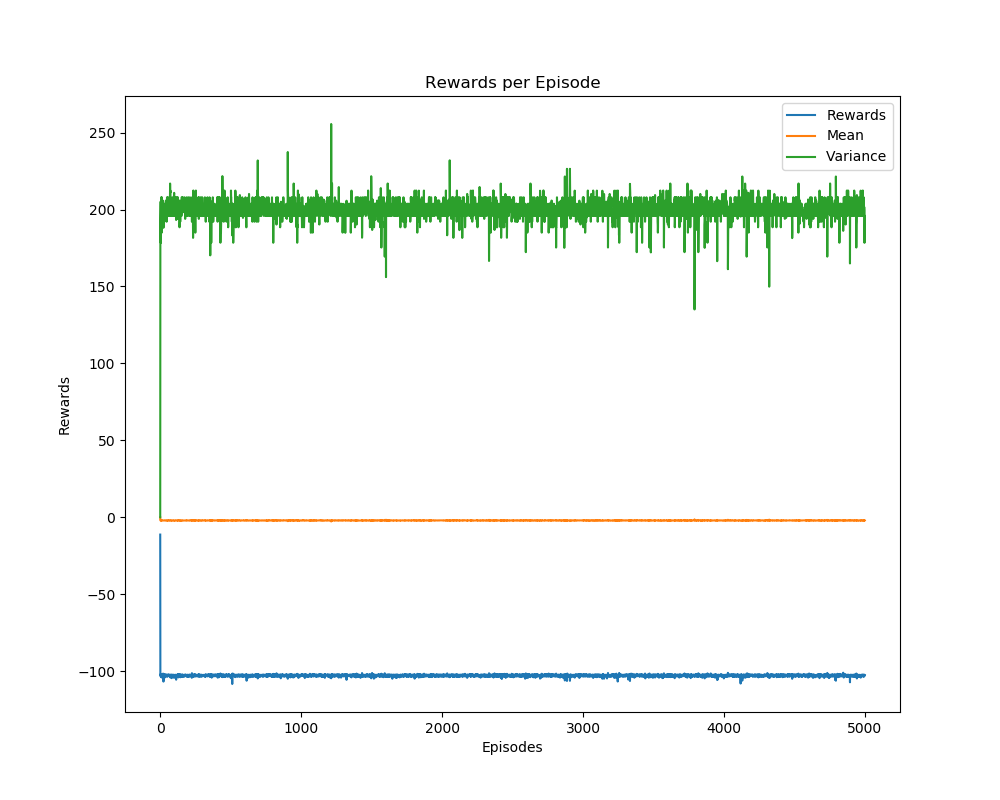
\includegraphics[width =\textwidth, height=0.4 \textheight]{results/ddpg/5000_ep/Rewards.png}
\caption{Reward when DDPG is run for 5000 Episodes}
\end{figure}

\begin{figure}
\label{DQN_5000Ep_Epsilon}
\includegraphics[width =\textwidth, height=0.4 \textheight]{results/ddpg/5000_ep/Epsilon.png}
\caption{Epislon when DDPG is run for 5000 Episodes}
\end{figure}
\FloatBarrier
\subsection{Comparison of DQN vs. DDPG}
The DDPG, while taking a lot more computational resources due to four different neural networks being utilized, does show steadier and more consistent results. While neither robotic walker completed the course, the DDPG walker had less \emph{very large} negative rewards (comparing figures \ref{DDPG_1000Ep_Rewards}  on page \pageref{DDPG_1000Ep_Rewards} vs figure \ref{DQN_1000Ep_Rewards} on page \pageref{DQN_1000Ep_Rewards}). This indicates that the LSTM used for action replay, as well as the critic network enabled a stabilization of the DDPG network that the DQN was otherwise unable to access. This can also be partially explained by the DQN using a more random $\epsilon$ rather than the smoothly-decaying $\epsilon$. We can see an extremely smooth graduation of the $\epsilon$ as seen in figure \ref{DDPG_1000Ep_Epsilon} on \pageref{DDPG_1000Ep_Epsilon} versus figure \ref{DQN_1000Ep_Epsilon} on page \pageref{DQN_1000Ep_Epsilon}. This implies that with sufficient computational power the DDPG would more smoothly get to a trained walker, as opposed to the DQN which has to rely much more on random exploration in order to determine an optimal strategy. 

Where the two diverge more absolutely is the training time each took. While it is roughly difficult to compare the two due to training occurring on a shared cluster, we saw the following approximate results:

\begin{tabular}{r||ll}
\hline 
\# Episodes & DQN & DDPG \\ 
\hline 
1000 &  \~ 20 minutes &  \~ 60 minutes \\ 
5000 & \~ 40 minutes & \~ 5 Hours \\ 
\hline
\end{tabular} 


The DDPG and DQN difference is not a linear difference, at least at the early stages but rather exponential. This is due to the DDPG using four different networks, the actor (agent) and critic (policy) networks, but also slowly decaying target networks for each. The DDPG also utilized a LSTM for the replay buffer, further increasing complexity as opposed to the DQN. 

For future iterations of this project, with a much larger and distributed computing cluster, the author would likely go with a DDPG network. However, to improve performance, the author would create two hyperparameters, a $\gamma$ and $\gamma^{\prime}$ for the local and target networks, respectively. During early stages of training $\gamma$ should be extremely low in order to  ensure the agent can operate. However, as time goes on, we would increase $\gamma$ so that $\lim_{t \to \infty} \gamma = 0.99$ with the $\gamma^{\prime}$ parameter scaling similarly. This is to ensure that in the long-run and the agent approaches a successful completion, they become more cautious and maximize reward output. 




\newpage 
\section{Concluding Remarks}

While we were ultimately unsuccessful  in getting the agent to complete the course, this research project was ultimately fruitful in understanding reinforcement learning, modifying code to successful execute reinforcement learning jobs, and yielding meaningful business value from future applications. 

First, a brief reflection on the epistemology of reinforcement learning and data science. Reinforcement learning theory does not formally fit into the epistemology of data science but is ultimately a successful tool for application of data science. While data science is fundamentally an empirical science since it uses existing data sets to design a model to predict future values or labels, data science has historically used heuristics and rational approaches. For example, while many data scientists can design a relatively useful credit card transaction fraud model, it takes deep expertise in the credit card industry to yield a well-turned model that fully takes advantage of most features. Indeed, deep learning is an attempt to make data science even more empirical by building feature engineering into an automatic function. Reinforcement learning, in contrast relies entirely on an \emph{environment}, or a model of an environment in order to yield knowledge making it an entirely rational endeavor. Deep applications to reinforcement learning yield an even more rational discipline since data scientists are no longer focusing on $\gamma$ discounting, game theory, and other intersections of mathematics and economics and rather on providing the most optimal environment. Ultimately, reinforcement learning attempts to create \emph{actions} which is a truly unique knowledge outcome across all studies of human knowledge and wisdom. The author predicts this will ultimately yield a bifurcation between data scientists and nascent applications for reinforcement learning, where the skillets are similar but the theory of knowledge differs completely. 

The author most regrets the lack of detailed coding for this practicum though still finds the experience rewarding. Ultimately, the base algorithms for DQN\citep{DQN_22} and DDPG\citep{DDPG} are open-sourced and implementations will not vary terribly much. As a result, the author largely took existing source code\footnote{https://github.com/Kyziridis/BipedalWalker-v2.git} and modified it to the needs of this project. This included the following items: \begin{enumerate*}
\item Helper code to save videos, if possible;
\item Tensorflow 1.0 vs. Tensorflow 2.0 compatibility, and;
\item Modification of neural networks architecture.
\end{enumerate*}. Unfortunately item 1 become largely inapplicable due to XServer configurations and inability to complete the course and item 2 was enough to get everything running. Ultimately this left item 3 as the most significant place where modifications could happen. Significant work was done on the DQN neural network with additional density layers and regularization, though this work was ultimately removed due to a corrupted save file (though the source still has these functions). Much more substantial work was done on the DDPG, but ultimately the model would not compile in the Tensorflow space. The author wishes to see this project more as an operational and research project, and will likely create fresh code over time. 



The business applications and value of reinforcement learning are potentially awesome. This is particularly true because business can be broken down into sub-components of reinforcement learning. A business will always have a state, either a balance sheet or a capture of the market, that can be encoded into reinforcement learning. Actions, or operations on their systems and process represents policy networks that we can train. Ultimately, since most profit functions from a business are necessarily convex (by standard definitions in economics) any business can use reinforcement learning to seek optimal market share in an arbitrary collection of other plays (the game), a market (the environment) and returns to their shareholders (the reward functions). Indeed, at the author's current company  we are already deep into the process of creating such a framework and have several research-partner institutions. The limiting factor is computational time. As the author experienced it takes a material investment in machines and power to yield a successful reinforcement learning model. 

Reinforcement learning is best encoded as a multi-agent game across a complex environment, meaning that a quantum strategy may work best for a solution \citep{Meyer:1999vs, Guo:2008kd}. The environment can be thought of an arbitrarily complex quantum system with the reward function established as a measure of the energy state of the environment, or the Hamiltonian. Since $\dim(\mathcal{A})=24$ for this environment, and $\dim(\text{Agent}) = \dim(\text{Actor}) \oplus \dim(\text{Critic}) = 106497 + 72836 = 179833$ we get that $\dim(\hat{H}) = \dim(\mathcal{A}) \otimes \dim(\text{Agent})  \approx 4.3 \times 10 ^{6}$. Roughly speaking, a 4.3 Mega-Qubit computer could solve the Bipedal walker. While Quantum-Computing and the necessary computing power are likely decades off, the intersection of deep reinforcement learning and quantum-mechanics could create truly unique business the exhibit the first facets of Strong-AI. 



\newpage
\bibliographystyle{apacite}
\cite{*}
\bibliography{TarlerPracticuum}

\end{document}
